\chapter{Evolução do ristretto} \label{ch:evolucao}

Grafos de colaboração do ristretto da versão 0.0.1 até a versão 0.0.21 gerados
com os dados extraidos pelo Doxyparse.

\begin{figure}[h]
\center
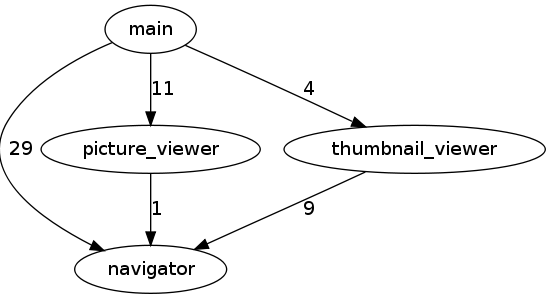
\includegraphics[scale=0.4]{imagens/ristretto-0_0_1-doxyparse-2}
\caption{ristretto 0.0.1}
\label{fig:ristretto-0.0.1-doxyparse-2-anexo}
\end{figure}

\begin{figure}[h]
\center
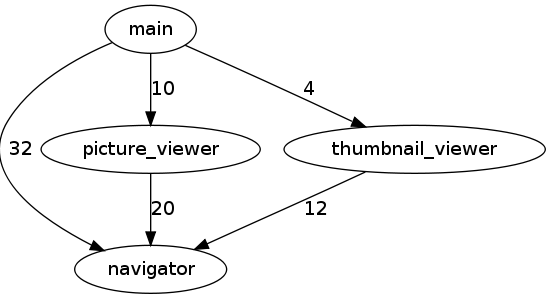
\includegraphics[scale=0.4]{imagens/ristretto-0_0_2-doxyparse-2}
\caption{ristretto 0.0.2}
\label{fig:ristretto-0.0.2-doxyparse-2-anexo}
\end{figure}

\begin{figure}[h]
\center
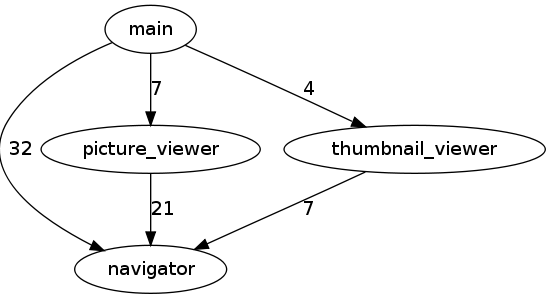
\includegraphics[scale=0.4]{imagens/ristretto-0_0_3-doxyparse-2}
\caption{ristretto 0.0.3}
\label{fig:ristretto-0.0.3-doxyparse-2-anexo}
\end{figure}

\begin{figure}[h]
\center
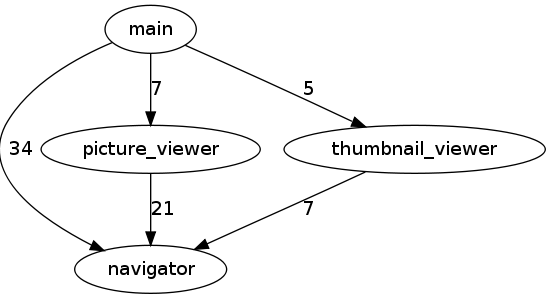
\includegraphics[scale=0.4]{imagens/ristretto-0_0_4-doxyparse-2}
\caption{ristretto 0.0.4}
\label{fig:ristretto-0.0.4-doxyparse-2-anexo}
\end{figure}

\begin{figure}[h]
\center
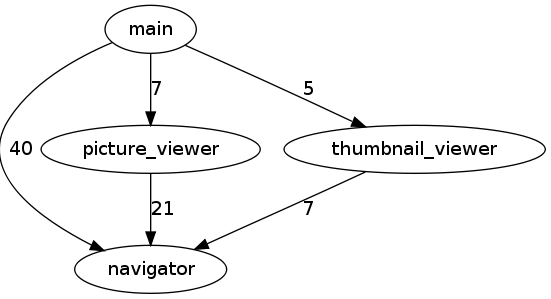
\includegraphics[scale=0.4]{imagens/ristretto-0_0_5-doxyparse-2}
\caption{ristretto 0.0.5}
\label{fig:ristretto-0.0.5-doxyparse-2-anexo}
\end{figure}

\begin{figure}[h]
\center
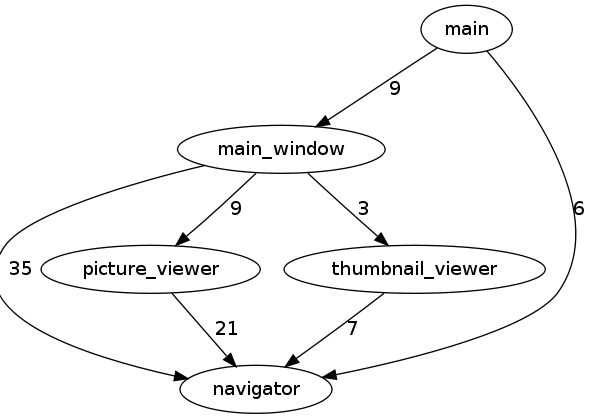
\includegraphics[scale=0.4]{imagens/ristretto-0_0_6-doxyparse-2}
\caption{ristretto 0.0.6}
\label{fig:ristretto-0.0.6-doxyparse-2-anexo}
\end{figure}

\begin{figure}[h]
\center
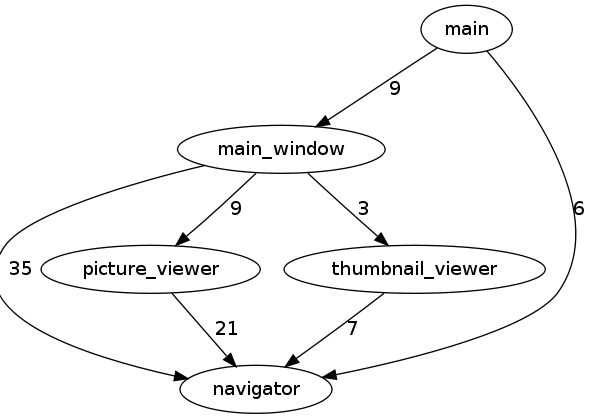
\includegraphics[scale=0.4]{imagens/ristretto-0_0_7-doxyparse-2}
\caption{ristretto 0.0.7}
\label{fig:ristretto-0.0.7-doxyparse-2-anexo}
\end{figure}

\begin{figure}[h]
\center
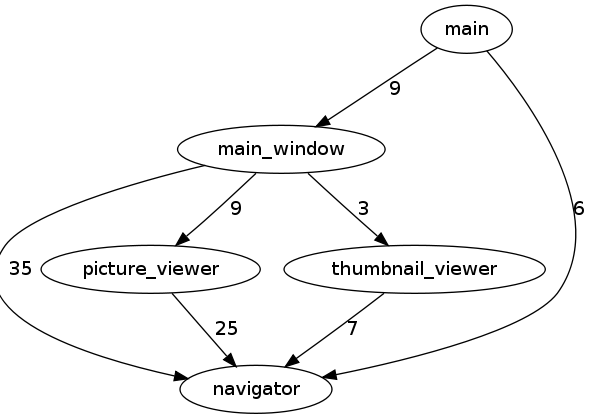
\includegraphics[scale=0.4]{imagens/ristretto-0_0_8-doxyparse-2}
\caption{ristretto 0.0.8}
\label{fig:ristretto-0.0.8-doxyparse-2-anexo}
\end{figure}

\begin{figure}[h]
\center
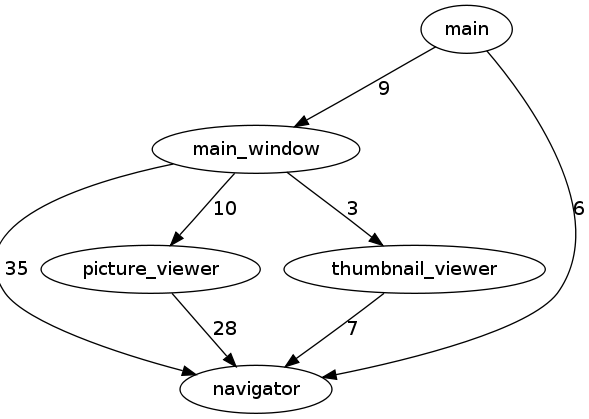
\includegraphics[scale=0.4]{imagens/ristretto-0_0_9-doxyparse-2}
\caption{ristretto 0.0.9}
\label{fig:ristretto-0.0.9-doxyparse-2-anexo}
\end{figure}

\begin{figure}[h]
\center
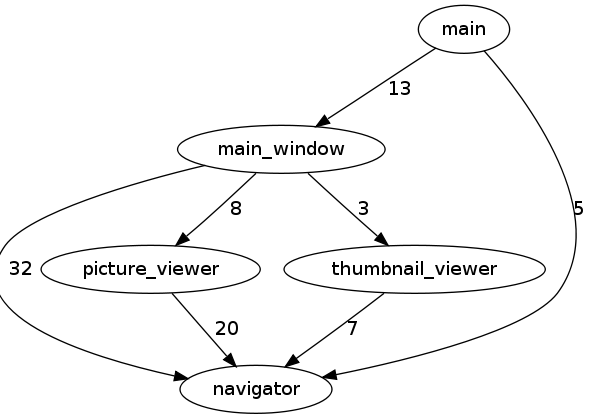
\includegraphics[scale=0.4]{imagens/ristretto-0_0_10-doxyparse-2}
\caption{ristretto 0.0.10}
\label{fig:ristretto-0.0.10-doxyparse-2-anexo}
\end{figure}

\begin{figure}[h]
\center
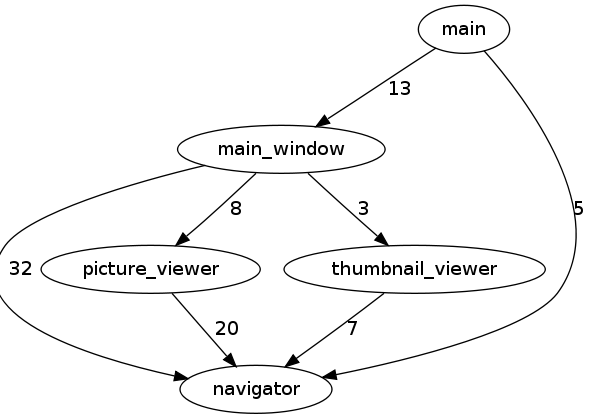
\includegraphics[scale=0.4]{imagens/ristretto-0_0_11-doxyparse-2}
\caption{ristretto 0.0.11}
\label{fig:ristretto-0.0.11-doxyparse-2-anexo}
\end{figure}

\begin{figure}[h]
\center
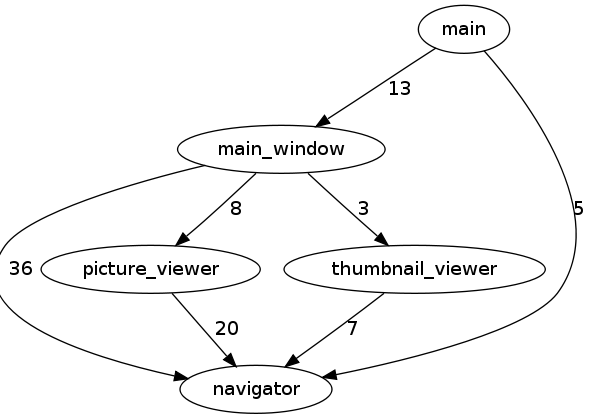
\includegraphics[scale=0.4]{imagens/ristretto-0_0_12-doxyparse-2}
\caption{ristretto 0.0.12}
\label{fig:ristretto-0.0.12-doxyparse-2-anexo}
\end{figure}

\begin{figure}[h]
\center
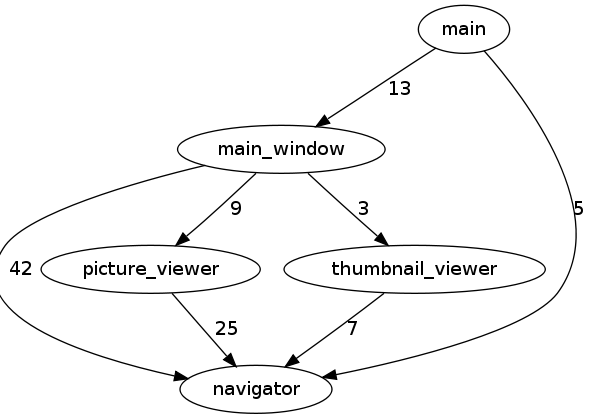
\includegraphics[scale=0.4]{imagens/ristretto-0_0_13-doxyparse-2}
\caption{ristretto 0.0.13}
\label{fig:ristretto-0.0.13-doxyparse-2-anexo}
\end{figure}

\begin{figure}[h]
\center
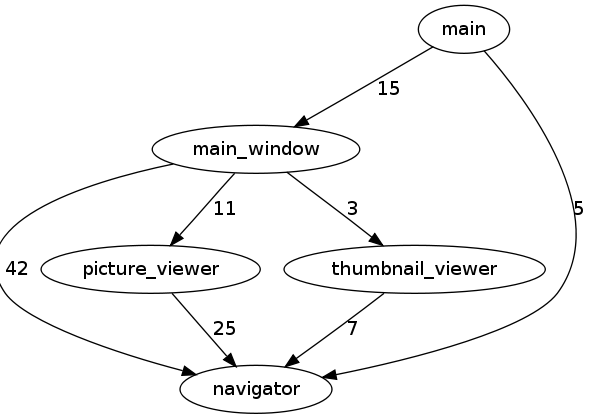
\includegraphics[scale=0.4]{imagens/ristretto-0_0_14-doxyparse-2}
\caption{ristretto 0.0.14}
\label{fig:ristretto-0.0.14-doxyparse-2-anexo}
\end{figure}

\begin{figure}[h]
\center
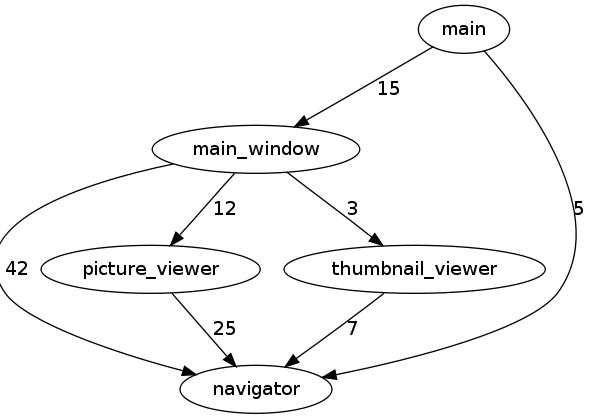
\includegraphics[scale=0.4]{imagens/ristretto-0_0_15-doxyparse-2}
\caption{ristretto 0.0.15}
\label{fig:ristretto-0.0.15-doxyparse-2-anexo}
\end{figure}

\begin{figure}[h]
\center
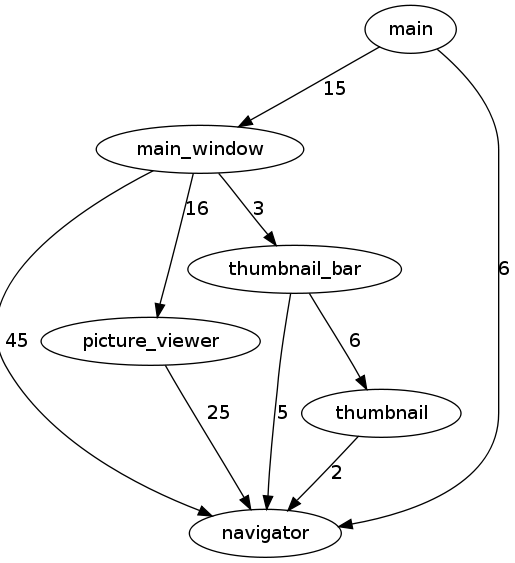
\includegraphics[scale=0.4]{imagens/ristretto-0_0_16-doxyparse-2}
\caption{ristretto 0.0.16}
\label{fig:ristretto-0.0.16-doxyparse-2-anexo}
\end{figure}

\begin{figure}[h]
\center
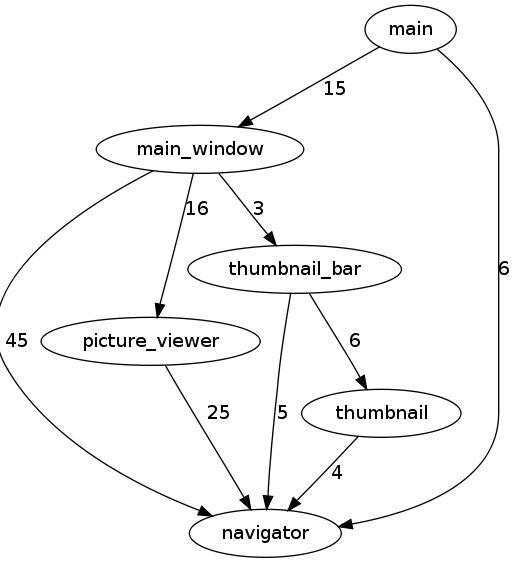
\includegraphics[scale=0.4]{imagens/ristretto-0_0_17-doxyparse-2}
\caption{ristretto 0.0.17}
\label{fig:ristretto-0.0.17-doxyparse-2-anexo}
\end{figure}

\clearpage % para evitar o erro: Too many unprocessed floats

\begin{figure}[h]
\center
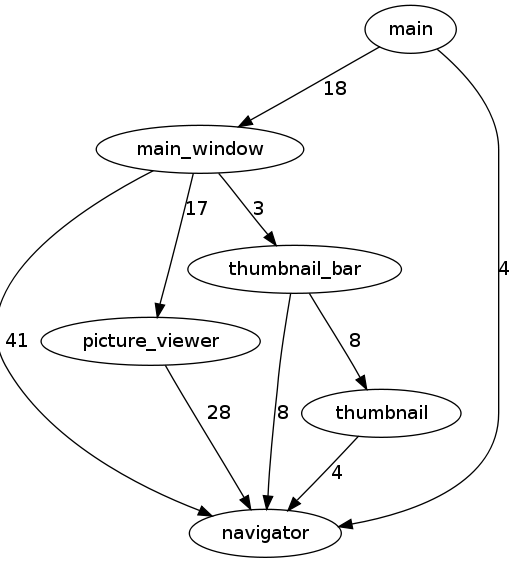
\includegraphics[scale=0.4]{imagens/ristretto-0_0_18-doxyparse-2}
\caption{ristretto 0.0.18}
\label{fig:ristretto-0.0.18-doxyparse-2-anexo}
\end{figure}

\begin{figure}[h]
\center
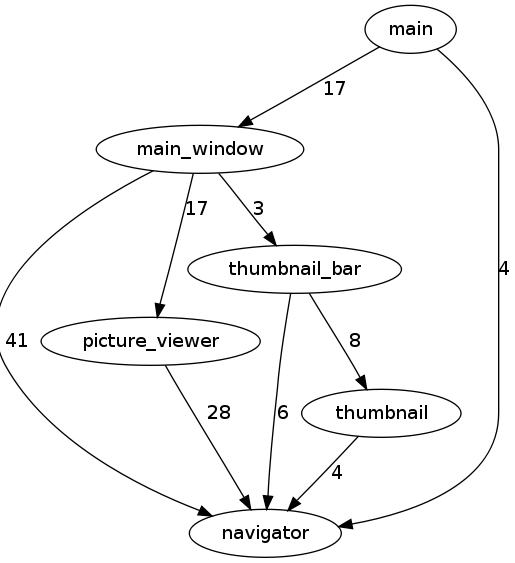
\includegraphics[scale=0.4]{imagens/ristretto-0_0_19-doxyparse-2}
\caption{ristretto 0.0.19}
\label{fig:ristretto-0.0.19-doxyparse-2-anexo}
\end{figure}

\begin{figure}[h]
\center
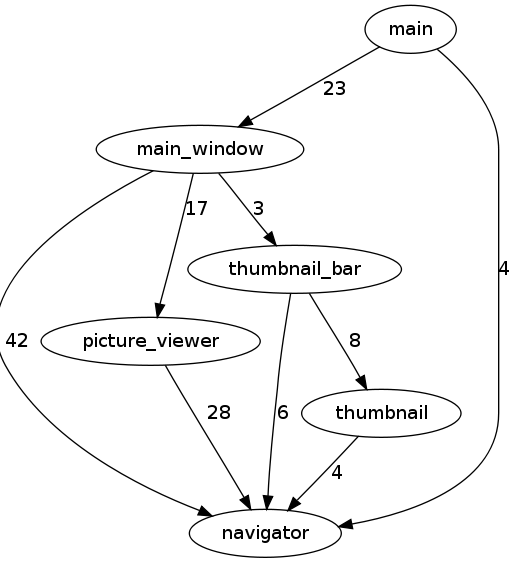
\includegraphics[scale=0.4]{imagens/ristretto-0_0_20-doxyparse-2}
\caption{ristretto 0.0.20}
\label{fig:ristretto-0.0.20-doxyparse-2-anexo}
\end{figure}

\begin{figure}[h]
\center
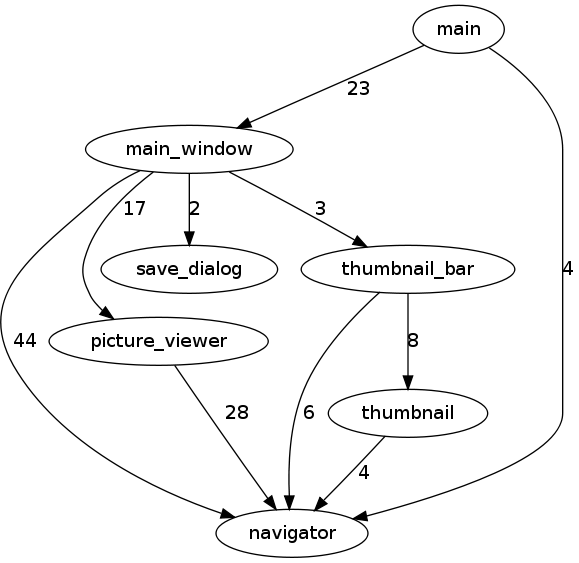
\includegraphics[scale=0.4]{imagens/ristretto-0_0_21-doxyparse-2}
\caption{ristretto 0.0.21}
\label{fig:ristretto-0.0.21-doxyparse-2-anexo}
\end{figure}

\chapter{Resumo de métricas do ristretto} \label{ch:resumo-comparativo}

\begin{table}
\caption{Resumo comparativo das métricas do ristretto atualizado}
\centering
\begin{tabular}{| l | c c | c c |}
\hline
Extrator  & \multicolumn{2}{|c|}{GCC}        & \multicolumn{2}{|c|}{Doxyparse} \\
\hline
Versão    & Falta de Coesão & Acoplamento    & Falta de Coesão & Acoplamento   \\
\hline
0.0.1     & 4.75            & 1.25           & 5.00            & 1.25          \\
0.0.2     & 5.75            & 1.25           & 6.00            & 1.25          \\
0.0.3     & 6.00            & 1.25           & 6.00            & 1.25          \\
0.0.4     & 6.25            & 1.25           & 6.25            & 1.25          \\
0.0.5     & 6.25            & 1.25           & 6.25            & 1.25          \\
0.0.6     & 7.60            & 2.20           & 7.60            & 1.40          \\
0.0.7     & 7.60            & 2.20           & 7.60            & 1.40          \\
0.0.8     & 7.00            & 2.20           & 7.20            & 1.40          \\
0.0.9     & 7.20            & 2.20           & 7.40            & 1.40          \\
0.0.10    & 7.60            & 2.20           & 8.00            & 1.40          \\
0.0.11    & 7.60            & 2.20           & 8.00            & 1.40          \\
0.0.12    & 7.60            & 2.20           & 8.00            & 1.40          \\
0.0.13    & 7.80            & 2.20           & 8.20            & 1.40          \\
0.0.14    & 8.00            & 2.20           & 8.40            & 1.40          \\
0.0.15    & 8.00            & 2.20           & 8.80            & 1.40          \\
0.0.16    & 7.16            & 2.33           & 7.83            & 1.50          \\
0.0.17    & 7.00            & 2.33           & 7.83            & 1.50          \\
0.0.18    & 7.50            & 2.16           & 8.33            & 1.50          \\
0.0.19    & 7.83            & 2.16           & 8.66            & 1.50          \\
0.0.20    & 8.83            & 2.16           & 10.00           & 1.50          \\
0.0.21    & 8.28            & 2.00           & 9.14            & 1.42          \\
\hline
\end{tabular}
\label{tab:comparacao-metricas-atualizada}
\end{table}
